\documentclass{article}

\usepackage{amsmath, amsthm, amssymb, amsfonts}
\usepackage{thmtools}
\usepackage{graphicx}
\usepackage{setspace}
\usepackage{geometry}
\usepackage{float}
\usepackage{hyperref}
\usepackage[utf8]{inputenc}
\usepackage[english]{babel}
\usepackage{framed}
\usepackage[dvipsnames]{xcolor}
\usepackage{tcolorbox}
\usepackage{textcomp}
\usepackage{listings} 


\colorlet{LightGray}{White!90!Periwinkle}
\colorlet{LightOrange}{Orange!15}
\colorlet{LightGreen}{Green!15}

\newcommand{\HRule}[1]{\rule{\linewidth}{#1}}

\declaretheoremstyle[name=Theorem,]{thmsty}
\declaretheorem[style=thmsty,numberwithin=section]{theorem}
\tcolorboxenvironment{theorem}{colback=LightGray}

\declaretheoremstyle[name=Proposition,]{prosty}
\declaretheorem[style=prosty,numberlike=theorem]{proposition}
\tcolorboxenvironment{proposition}{colback=LightOrange}

\declaretheoremstyle[name=Principle,]{prcpsty}
\declaretheorem[style=prcpsty,numberlike=theorem]{principle}
\tcolorboxenvironment{principle}{colback=LightGreen}

\setstretch{1.2}
\geometry{
    textheight=9in,
    textwidth=5.5in,
    top=1in,
    headheight=12pt,
    headsep=25pt,
    footskip=30pt
}

\begin{document}

% ====== TITLE PAGE ======
\title{ \normalsize \textsc{}
		\\ [2.0cm]
		\HRule{1.5pt} \\
		\LARGE \textbf{\uppercase{[Project 2]}
		\HRule{2.0pt} \\ [0.6cm] \LARGE{[AI6126 : Advanced Computer Vision]} \vspace*{5\baselineskip}}
		}
\date{[26 April 2023]}
\author{\textbf{Riemer van der Vliet} \\ 
    G2304212K}

\maketitle

\newpage

% ====== GENERIC SECTION TEMPLATE ======
\section{introduction}
\label{sec:introduction} % Label for referencing

The goal of this mini-challenge is to generate high-quality (HQ) face images from the
corrupted low-quality (LQ) ones (see Figure 1) [1]. The data for this task comes from
the FFHQ. For this challenge, we provide a mini dataset, which consists of 5000 HQ
images for training and 400 LQ-HQ image pairs for validation. Note that we do not
provide the LQ images in the training set.
% Subsection example

\subsection{dataset}
\label{subsec:dataset} % Label for referencing

\subsection{evaluation}



\section{Other Models}
\label{sec:otherModels} % Label for referencing

This section presents an overview of other influential models and techniques in the field of super-resolution, particularly focusing on the innovations brought by BasicSR and Real-ESRGAN. These techniques offer alternative methods to achieve high-quality image super-resolution.

\subsection{Techniques from BasicSR}
\label{subsec:BasicSR} % Label for referencing

BasicSR introduces several key techniques that enhance the quality of super-resolution outputs:

\begin{itemize}
    \item \textbf{SRResNet:} This baseline architecture utilizes residual blocks to achieve effective super-resolution without extensive computational costs.
    \item \textbf{Perceptual Loss:} Unlike traditional loss functions like MSE, BasicSR employs perceptual loss that uses pretrained neural networks (e.g., VGG) to assess perceptual similarity between images, which often leads to more visually pleasing results.
    \item \textbf{Feature Fusion:} This technique allows the model to integrate and leverage information from multiple scales or network branches, enhancing the detail and quality of the upsampled images.
\end{itemize}

\subsection{Techniques from Real-ESRGAN}
\label{subsec:Real-ESRGAN} % Label for referencing

Real-ESRGAN advances super-resolution through several sophisticated architectural improvements:

\begin{itemize}
    \item \textbf{Enhanced Residual Dense Network (ERDN):} This architecture combines the strengths of residual and dense networks to improve image detail and texture in super-resolution tasks.
    \item \textbf{Adaptive Instance Normalization (AdaIN):} Used within the network, AdaIN adjusts the style of features dynamically, contributing to the flexibility and effectiveness of the super-resolution process.
    \item \textbf{Attention Mechanisms:} By incorporating attention mechanisms, Real-ESRGAN can focus more on significant regions of the image, thus prioritizing areas that most impact perceptual quality.
\end{itemize}

It is crucial to recognize that in super-resolution, the highest scores are often achieved not by merely producing visually appealing images but by optimizing for metrics such as the Peak Signal-to-Noise Ratio (PSNR). This metric critically influences model performance evaluation in this domain.
\section{Results}
\label{sec:results} % Label for referencing

In this mini-challenge, our objective was to generate high-quality (HQ) face images from corrupted low-quality (LQ) ones using the Real-ESRGAN model. Below we present some example outputs along with the loss curves observed during training.

\begin{figure}[htbp]
    \centering
    \begin{minipage}{0.45\textwidth}
        \centering
        
\includegraphics[width=\textwidth]{imgs/output_00328.png}
        \caption{Example of HQ image generated from LQ input.}
        \label{fig:image1}
    \end{minipage}\hfill
    \begin{minipage}{0.45\textwidth}
        \centering
        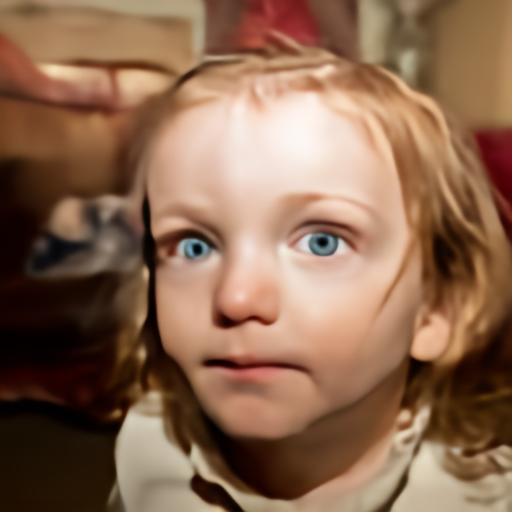
\includegraphics[width=\textwidth]{imgs/output_00386.png}
        \caption{Another example of enhanced HQ output.}
        \label{fig:image2}
    \end{minipage}
\end{figure}

\begin{figure}[htbp]
    \centering
    \begin{minipage}{0.45\textwidth}
        \centering
        
\includegraphics[width=\textwidth]{imgs/00328.png}
        \caption{Further illustration of HQ output from Real-ESRGAN.}
        \label{fig:image3}
    \end{minipage}\hfill
    \begin{minipage}{0.45\textwidth}
        \centering
        
\includegraphics[width=\textwidth]{imgs/00386.png}
        \caption{Additional HQ image showcasing model capabilities.}
        \label{fig:image4}
    \end{minipage}
\end{figure}

\begin{figure}[htbp]
    \centering
    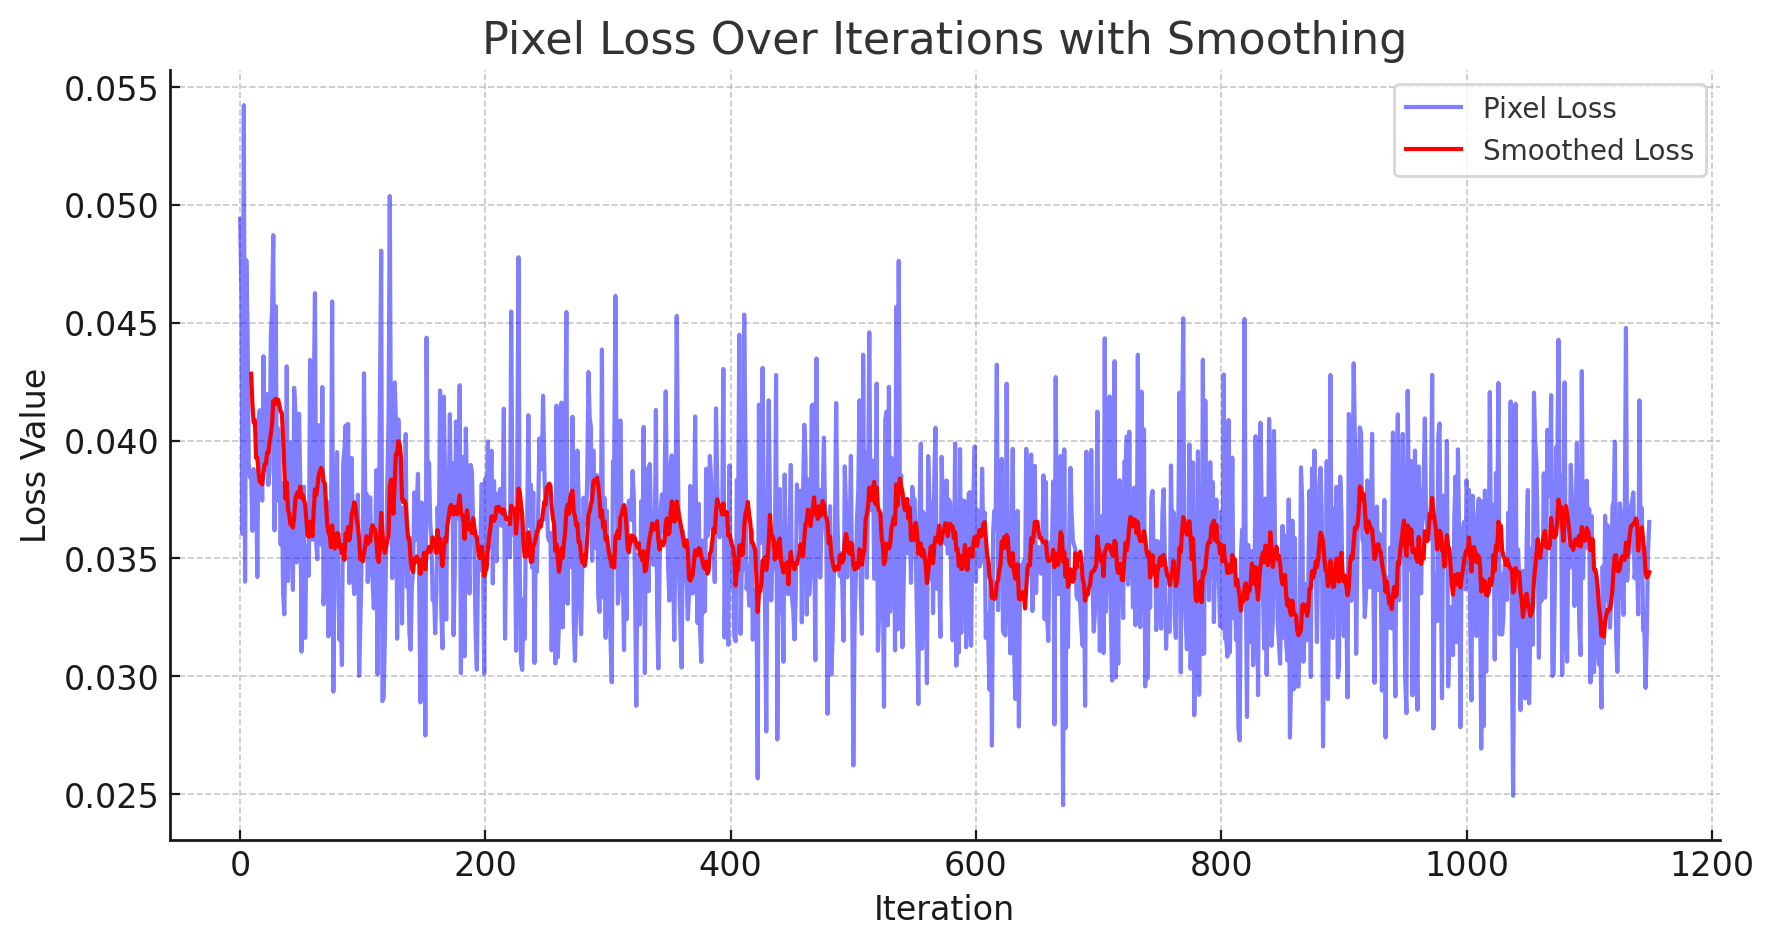
\includegraphics[width=\textwidth]{imgs/losses.png}
    \caption{Training loss curves over 115,000 iterations.}
    \label{fig:image5}
\end{figure}

These results were achieved after training the model on the NTU GPU cluster using an A40 GPU for 115,000 iterations—the maximum allowed training duration. The model reached a Peak Signal-to-Noise Ratio (PSNR) score of $26.40953$ in the blind test, demonstrating the effectiveness of the Real-ESRGAN model in enhancing image quality from LQ inputs. Detailed settings used during the training are provided in the appendix.

\section{Discussion}
\label{sec:Discussion} % Label for referencing

This project brings to light the delicate balance required in super-resolution between optimizing for human visual preferences and computational metrics. While human observers prioritize perceptual and semantic details, computational models tend to focus on precise pixel-based evaluations.

The use of Generative Adversarial Networks (GANs) equipped with perceptual loss functions is a promising approach to reconcile these perspectives. Perceptual loss allows for the generation of images that are more visually pleasing to humans by mimicking the way human vision processes images. However, this often results in lower Peak Signal-to-Noise Ratio (PSNR) scores, as the focus shifts from exact pixel accuracy to more qualitative aspects of image quality.

Despite the potential benefits of perceptual loss, it was not utilized in this experiment due to constraints on using external data. Understanding that the highest PSNR scores do not always correlate with the most visually appealing images is crucial. 


\section{References}

Please find the git repository for this project~\href{https://github.com/Riemer1818/AI6126-AdCV-Proj2}{AI6126-AdCV-Proj2}

Please find the git repository for REAL-ESRGAN~\href{https://github.com/xinntao/Real-ESRGAN}{Real-ESRGAN}

Please find the git repository for BasicSR~\href{https://github.com/XPixelGroup/BasicSR}{BasicSR}

\end{document}